\section{Related Work}
\label{sec:related}

\subsection{Explainability and counterfactual model probing}

Many post-hoc image explanations assign importance to pixels or regions. Their reliability depends on whether the explanation actually changes with the learned model, a point made explicit by saliency-map sanity checks~\cite{adebayo2018sanity} and by work on explainability in precision pathology~\cite{klauschen2024xai}. Counterfactual explanations take a different form: they search for a nearby input with a different prediction. Goyal \etal{} use discriminative visual comparisons~\cite{goyal2019counterfactual}. DVCE and DiME place classifier-guided edits under diffusion image priors~\cite{augustin2022dvce,jeanneret2022dime}, and DiG-IN extends diffusion guidance to comparisons between networks and neuron-level visualization~\cite{augustin2024digin}.

Interventions have also been used to examine the generative model itself. Tinaz \etal{} fit sparse autoencoders to diffusion activations, identify concepts at different denoising stages, and manipulate image composition and style through those concepts~\cite{tinaz2025concepts}. This line of work is useful for understanding where a generative representation forms. Our experiments instead use a conditional generator as an input instrument for testing external pathology models.

In histopathology, synthetic class transitions have revealed patterns associated with molecular labels~\cite{dolezal2023synthetic}. MoPaDi couples a diffusion autoencoder~\cite{preechakul2022diffae} to classifiers and multiple-instance models, then edits morphology toward a target prediction~\cite{zigutyte2026mopadi}. \method{} fixes the cellular intervention before querying the downstream model. Selection is based on recovered condition fidelity, so the same pair can be shown to several architectures.

\subsection{Pathology representations and cellular analysis}

TCGA made matched pathology and molecular data available across tumor types and institutions~\cite{tcga2013pancancer}. CTransPath introduced transformer-based contrastive pretraining for histopathology~\cite{wang2022ctranspath}. UNI and Virchow later scaled visual pretraining to larger slide collections~\cite{chen2024uni,vorontsov2024virchow}; CONCH added image--language supervision~\cite{lu2024conch}; and Prov-GigaPath modeled long-range WSI context~\cite{xu2024gigapath}. We treat these encoders as models to audit with controlled inputs. Their pretraining scale alone does not indicate whether a downstream response comes from morphology, cell layout, stain, or another feature.

The controls and measurements in this paper depend on cell-level structure. HoVer-Net jointly segments and classifies nuclei in multi-tissue histology~\cite{graham2019hovernet}. StarDist detects instances using star-convex polygons~\cite{schmidt2018stardist}, while CellViT++ combines a foundation-model encoder with efficient cell segmentation and classification~\cite{horst2026cellvitpp}. These models disagree in taxonomy and boundary placement. We use that disagreement deliberately: CellViT++ participates in candidate selection, while HoVer-Net and StarDist provide out-of-loop measurements.

\subsection{Controllable histopathology generation}

PathologyGAN learned realistic tissue structure and interpretable latent representations with a generative adversarial model~\cite{quiros2021pathologygan}. PathLDM introduced text-conditioned latent diffusion for histopathology patches~\cite{yellapragada2024pathldm}; Harb \etal{} extended diffusion synthesis to gigapixel WSIs~\cite{harb2024gigapixel}; and Spatial Diffusion modeled explicit cell layouts~\cite{li2024spatialdiffusion}. CPathOGen focuses on paired samples for which a requested cellular or appearance change can be recovered from the output.

The architecture uses latent diffusion to perform denoising in a compressed image representation~\cite{rombach2022latent}. A ControlNet branch supplies the dense cellular map~\cite{zhang2023controlnet}. FiLM layers apply condition-dependent scale and shift throughout the denoising network~\cite{perez2018film}. Local organization and global morphology therefore enter through separate paths: five spatial channels carry cellular position, and a global vector carries geometry, texture, and RGB statistics.

\subsection{Realism, condition fidelity, and auditing}

FID~\cite{heusel2017fid} and KID~\cite{binkowski2018kid} compare generated and reference feature distributions. Neither metric tests adherence to a spatial map or morphology vector. A generator can score well while placing the wrong cell type, missing a requested count, or changing stain together with nuclear shape.

We report realism and condition fidelity separately. Spatial checks use recovered counts and centroid agreement. Morphology is measured across images and again within the same source image over a five-level dose sweep. Downstream probing is restricted to pairs that pass the generation-side checks. Figure~\ref{fig:overview} shows where selection and independent auditing enter the pipeline.

\begin{figure*}[!t]
    \centering
    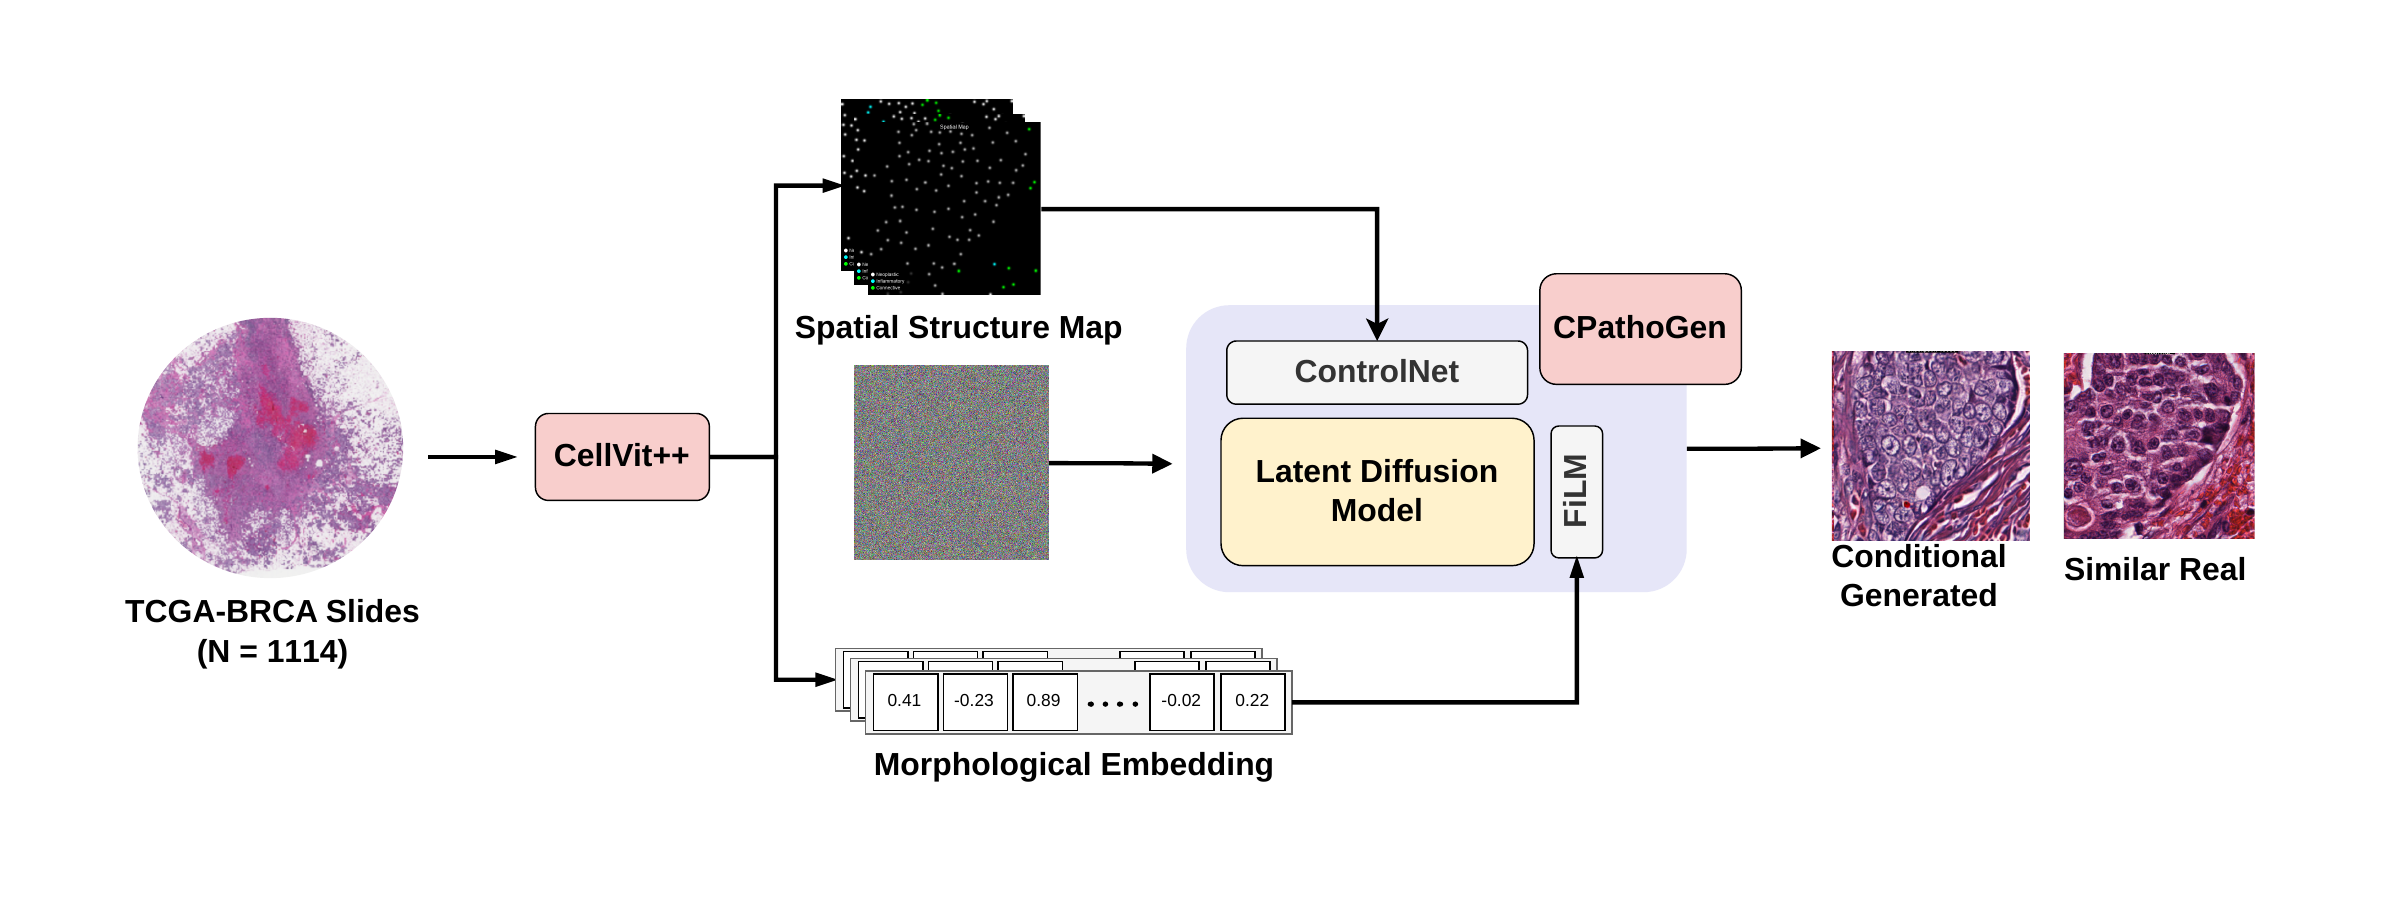
\includegraphics[width=\textwidth,height=0.30\textheight,keepaspectratio]{related_work/cpathogen_overview.png}
    \vspace{-12mm}
    \caption{\method{} synthesis, selection, auditing, and model probing.}
    \label{fig:overview}
\end{figure*}
